Having presented ... ,
\todo{add intro}
% the goal of this chapter is to demonstrate the use of the proposed query processing architecture in ...
% More specifically, we present case studies ...
% we apply 

\section{Flexible secondary index partitioning}
In section~\ref{sec:index_partitioning_background} we described the most common techniques for partitioning a secondary index:
\begin{itemize}
  \item \textbf{Partitioning by document}.
  Each index partition is responsible for the data items of a corpus partition,
  and is co-located in the same node as that corpus partition.
  \item \textbf{Partitioning by term}.
  Each index partition is responsible for a part of the \textit{value space} of the indexed attribute,
  and its placement is independent from the corresponding corpus partition.
\end{itemize}

Experimental comparison of the two approaches has shown \cite{dsilva:tworings, kejriwal:slik} that there is no ``one-size-fits-all'' approach to secondary
index partitioning.
Rather, each approach caters to different needs.
More specifically, partitioning by document is more suitable for:
\begin{itemize}
  \item Workloads with low selectivity queries, that return large result sets.
  \item Corpora with skewed indexed attribute distributions (a large number of data items correspond to a few attribute values).
  \item Write-intensive workloads that require low update latency.
\end{itemize}
\noindent
On the other hand, partitioning by term is more suitable for:
\begin{itemize}
  \item Large-scale systems with a large number of corpus partitions.
  \item High selectivity query workloads.
  \item Corpora with normal indexed attribute distributions.
\end{itemize}

Therefore, the decision about which approach to be used for an index should be based on the corpus and the workload characteristics.

In most existing system, the choice of index partitioning scheme is made during the system's design phase, and is therefore \textit{static}.
For example, MongoDB \cite{coubase:mongoindexes}, Cassandra \cite{cassandra:secondaryindexing} and Riak \cite{riakv:secondaryindexes}
use the partitioning by document approach,
while HBase \cite{hbase:secondaryindexes} uses the partitioning by term approach.

\bigskip
\noindent
In this section, we demonstrate the flexibility of QPU query processing architecture by showing how it can be used to
express both index partitioning schemes.
The design of the QPU architectures is based on observations about the properties of the alternative
index partitioning schemes.
We categorize these observations using the derived state read and write path framework presented in
section~\ref{sec:read_write_path}:
\begin{itemize}
  \item In partitioning by document, the index \textbf{write path} is \textit{local}:
  an index partition receives updates only from the corpus partition with which it is co-located.
  On the hands, in partitioning by term, the write path involves a many-to-one relationship:
  an index partition receives updates from all corpus partitions, corresponding to the value interval it is responsible for.

  \item In partitioning by document, the \textbf{read path} is a \textit{broadcast} operation:
  a query is forwarded to all index partitions.
  On the other hand, in partitioning by term, only index partitions with relevant index terms are involved in processing a given query.
\end{itemize}

We present QPU architectures for the two index partitioning approaches using the photo album example of section~\ref{sec:read_write_path} as a reference.
The corpus is composed of a set of image files, and each image can be associated with user-defined tags.
The corpus is partitioned using a hash of the primary key as partitioning key.
An application needs to create a secondary index on the $predominantColor$ tag, which can be assigned values in the range $[\#000000$, $\#FFFFFF$].

Figures~\ref{fig:index_partitioned_by_document} and~\ref{fig:index_partitioned_by_term} show the QPU graphs and their
placement across system nodes for a document-partitioned index and a term-partitioned index respectively.
For simplicity we assume that the number of corpus partitions is equal to the number of system nodes,
and that a corpus partition is placed on each node.

In both architectures, an index QPU is used to represent each index partition;
A partition manager QPU, connected to all index partitions, and is responsible for coordinating query access to them.
Moreover, a corpus driver QPU is placed on each node, and is responsible for the data items of the corpus
partition it is co-located with.

\subsection{Write path}

\begin{figure}
  \begin{minipage}{.5\textwidth}
    \centering
    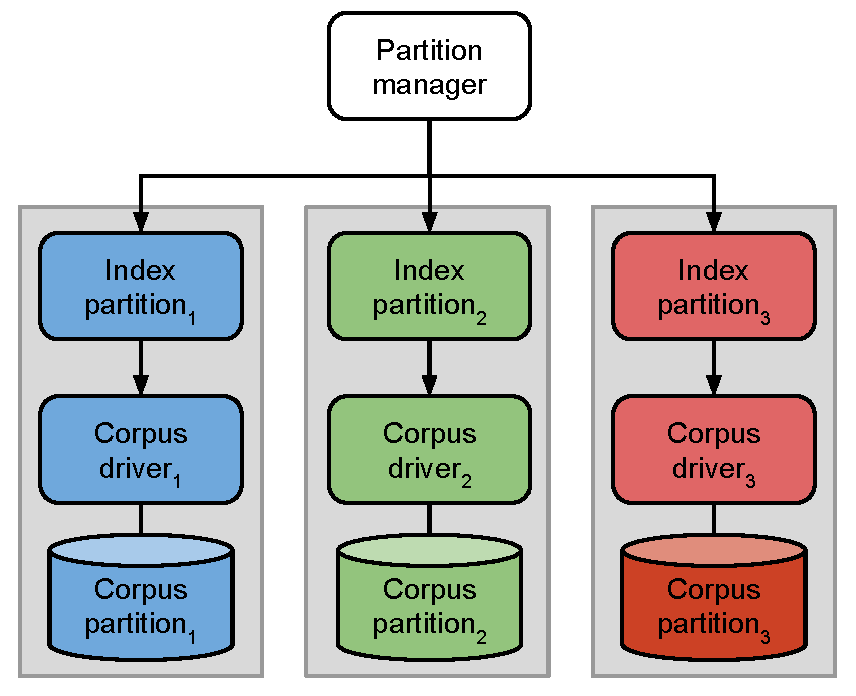
\includegraphics[scale=0.5]{./figures/case_studies/index_partitioned_by_document.pdf}
    \caption{QPU architecture for a document-partitioned secondary index.}
    \label{fig:index_partitioned_by_document}
  \end{minipage}%
  \begin{minipage}{.5\textwidth}
    \centering
    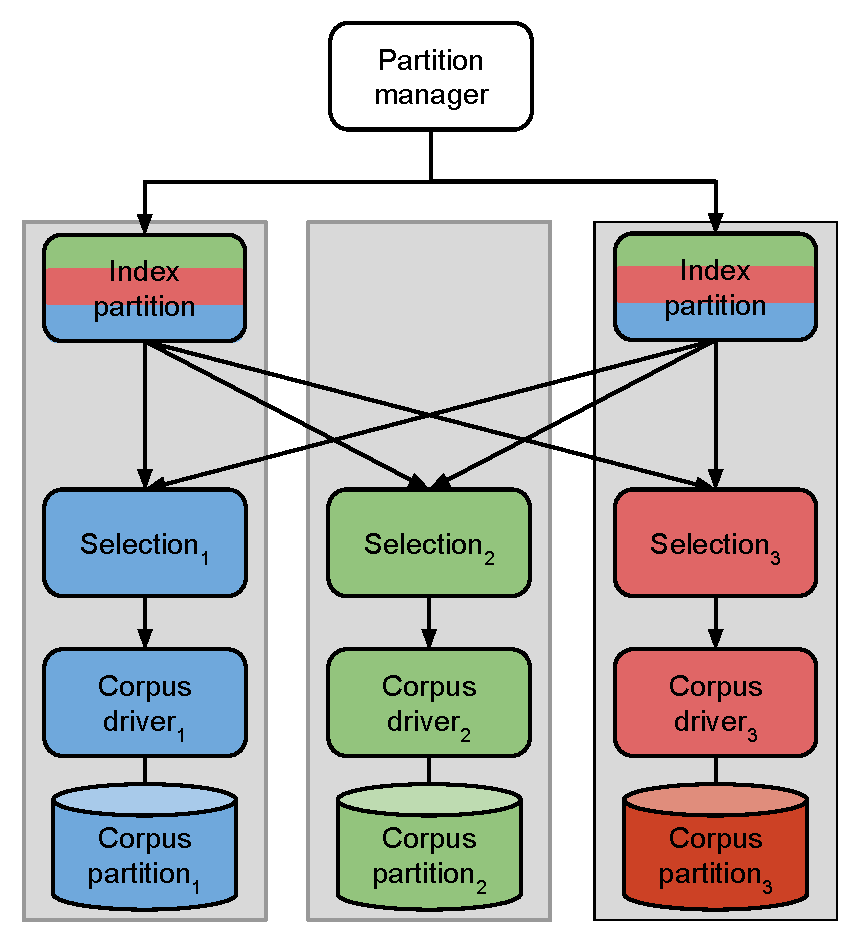
\includegraphics[scale=0.5]{./figures/case_studies/index_partitioned_by_term.pdf}
    \caption{QPU architecture for a term-partitioned secondary index.}
    \label{fig:index_partitioned_by_term}
  \end{minipage}
\end{figure}

The write path properties described above are achieved through (1) the QPU graph topology and the placement of graph vertices across system nodes,
and (2) the configuration of the index QPUs (index partitions).

\subsubsection{Graph topology and placement}

\medskip
\noindent
\textbf{Partitioning by document.}
In the partitioning by document approach, an index partition is placed on each system node, and is connected to the
corresponding corpus driver.
Therefore, each index partition communicates only with the corpus driver it is co-located with.

\medskip
\noindent
\textbf{Partitioning by term.}
In the partitioning by term approach, index partitions can be flexibly placed across nodes.
Each index partition is connected to all corpus driver QPUs, because an index partition is responsible for data
items in all corpus partitions.
Moreover, a filter QPU is connected to each corpus driver.
This permits each update to be forwarded to the relevant index partition based on the attribute value in the update.

\subsubsection{Index partition configuration and graph initialization}

When the QPU graph for one of the partitioned index architectures is initialized,
the initialization function of each index partition sends interval queries to the QPU's downstream connections,
in order to establish an input stream of updates.
The initialization function uses the index QPU's \textit{configuration} to generate the appropriate query request for each
downstream connection.
More specifically, each index QPU is configured with an attribute ($predominantColor$ in this example),
and an \textit{interval of values} of that attribute.
The index partition is responsible for index entries that correspond to attribute values in the specified interval.

\medskip
\noindent
In the partitioning by document approach,
all index partitions are configured to be responsible for the entire attribute value space,
which in the photo album example is $[\#000000$, $\#FFFFFF$].
Conversely, in the partitioning by term approach, each index partition is responsible for a non-overlapping subset of the
attribute value space.
A simplified version of the configuration of the index partitions of the term-partitioned index QPU architecture
(figure~\ref{fig:index_partitioned_by_term}) is depicted below: \\

% \noindent
\begin{minipage}{.48\textwidth}
\begin{lstlisting}[caption={Configuration of $index_1$ in Figure~\ref{fig:index_partitioned_by_term}},captionpos=b,frame=tlrb]{Name}
{
  // other configuration
  // parameters
  "indexConfiguration": {
    "table": "photoAlbum",
    "attribute":
        "predominantColor",
    "lower_bound": #000000,
    "upper_bound": #7FFFFF
  }
}
\end{lstlisting}
\end{minipage}\hfill
\begin{minipage}{.48\textwidth}
\begin{lstlisting}[caption={Configuration of $index_2$ in Figure~\ref{fig:index_partitioned_by_term}},captionpos=b,frame=tlrb]{Name}
{
  // other configuration
  // parameters
  "indexConfiguration": {
    "table": "photoAlbum",
    "attribute":
        "predominantColor",
    "lower_bound": #7FFFFF,
    "upper_bound": #FFFFFF
  }
}
\end{lstlisting}
\end{minipage}

\noindent
In the case of the document partitioned index architecture, all index partitions have the same ``indexConfiguration'' with
$lower_bound$ $=$ $\#000000$ and $higher_bound$ $=$ $\#FFFFFF$.
Therefore, in the \textbf{document-partitioned} index architecture, upon initialization, each index partition sends the query \\
{\obeylines\obeyspaces
  SELECT primaryKey, predominantColor
  FROM photoAlbum
  INTERVAL FROM LATEST
} ~\\
to the corpus driver it is connected to.
This establishes a stream between each corpus driver and the corresponding index QPU, through which the corpus driver
sends to the index QPU notifications for updates to the data item of the corpus partition it responsible for,
which the required read path behavior for the document-partitioned index.

\medskip
\noindent
In the \textbf{term-partitioned} index architecture, upon initialization, $index_1$ sends the query \\
{\obeylines\obeyspaces
    SELECT primaryKey, predominantColor
    FROM photoAlbum
    WHERE predominantColor $\geq$ $\#000000$ AND predominantColor $<$ $\#7FFFFF$
    INTERVAL FROM LATEST
} ~\\
to each filter QPU it is connected to, and $index_2$ \\
{\obeylines\obeyspaces
  SELECT primaryKey, predominantColor
  FROM photoAlbum
  WHERE predominantColor $\geq$ $\#7FFFFF$ AND predominantColor $leq$ $\#FFFFFF$
  INTERVAL FROM LATEST
} ~\\
to each of its downstream connections.

\noindent
Each filter QPU in turn establishes for each received query, an input stream of data item from the corpus partition it
is connected to, by sending the query: \\
{\obeylines\obeyspaces
  SELECT primaryKey, predominantColor
  FROM photoAlbum
  INTERVAL FROM LATEST
} ~\\
As a result, updates on data items of each corpus partition are sent from the corpus driver to the filter QPU corresponding
to that partition.
The filter QPU forwards each update to the corresponding index partition, based on the attribute value in the update.
This achieves the required write path functionality for the term-partitioned index.

For example, as a result of the creation of an image file with $predominantColor$ $=$ $\#613930$, assigned to to $corpus$
$partition_2$, $corpus$ $driver_2$ sends to $filter_2$ a record encoding that update.
This input record matches the query \\
{\obeylines\obeyspaces
    SELECT primaryKey, predominantColor
    FROM photoAlbum
    WHERE predominantColor $geq$ $\#000000$ AND predominantColor $<$ $\#7FFFFF$
    INTERVAL FROM LATEST
} ~\\
and thus the filter QPU sends the update record only to the $index_1$ partition.

\subsection{Read path}
In both QPU architectures, the partition manager QPU is connected to all index partitions.
As described in section~\ref{sec:qpc_tree}, given a query,
the partition manager's query processing function determines which index partitions need to be contacted and generates
the corresponding queries, using the query processing capabilities trees of its downstream connections.

More specifically, the query processing function, performs an ``intersection'' between the query parse tree
and the QPC tree of each of its downstream connections.
The result of each intersection operation is a query parse tree representing the downstream query that the partition manager
needs to send to the corresponding index QPU.
If the intersection result is empty, then no query needs to be sent by the partition manager to the corresponding
connection.

\begin{figure}
  \centering
    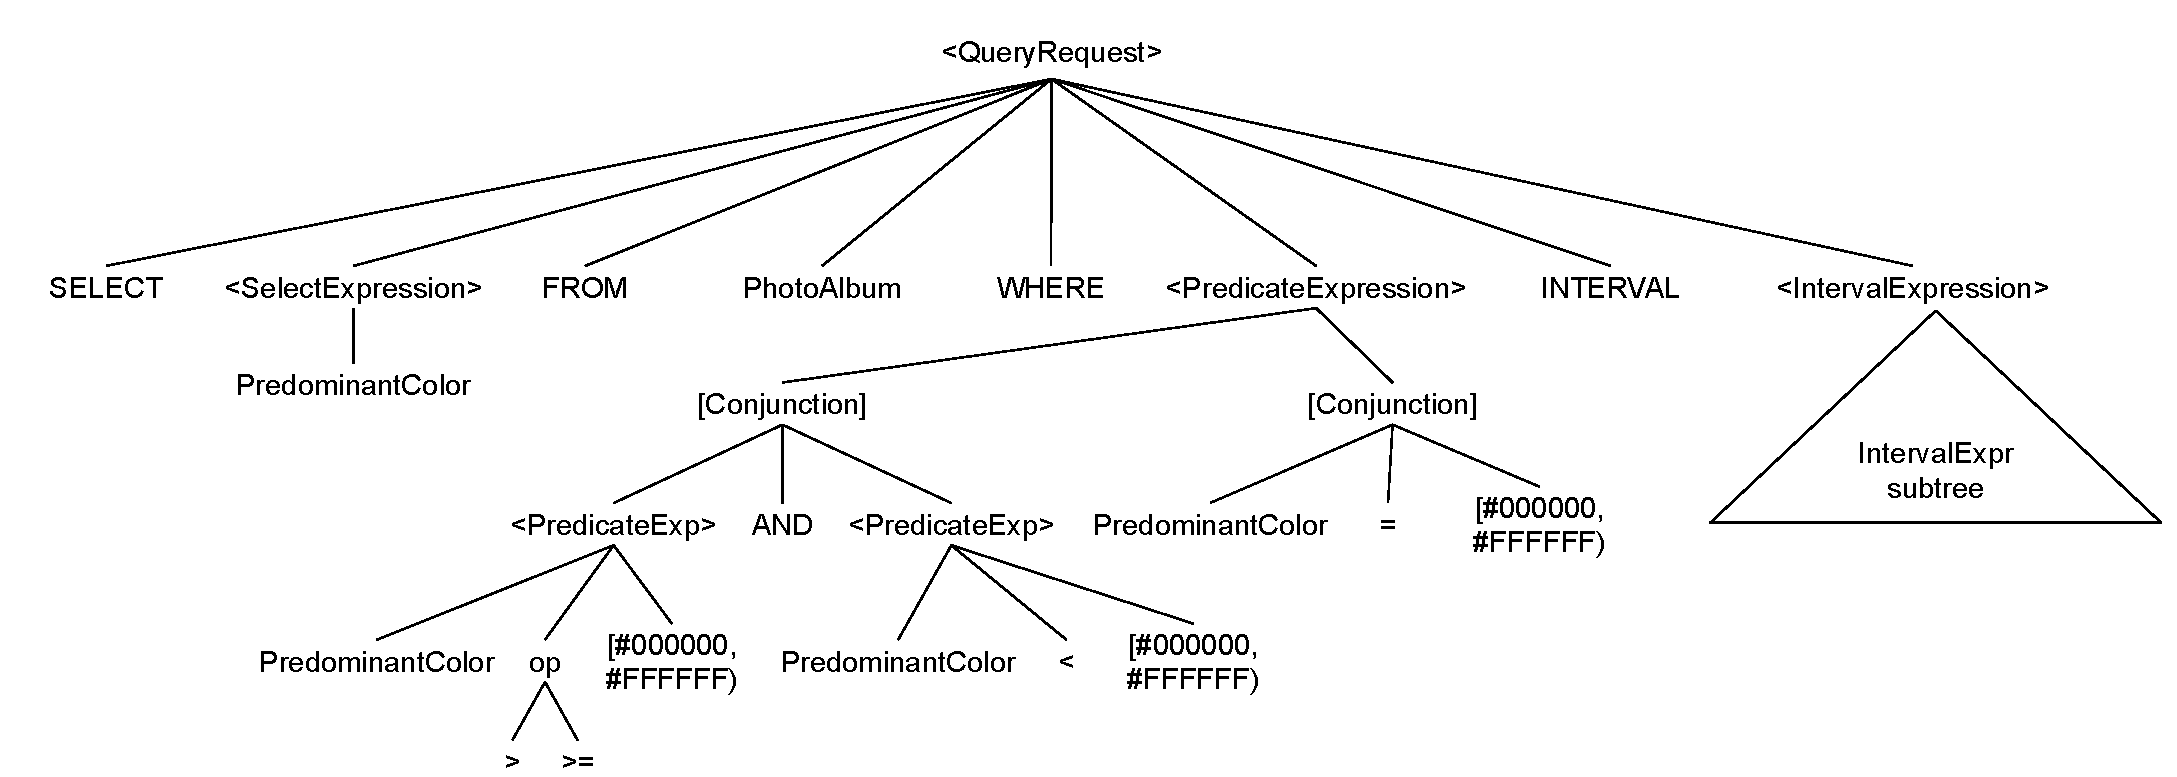
\includegraphics[width=\textwidth]{./figures/case_studies/qpt_index_partitioning_docs.pdf}
  \caption{Query processing tree of an index partition in the document-partitioned index QPU architecture.}
  \label{fig:qpt_index_partitioning_docs}
\end{figure}

\medskip
\noindent
\textbf{Partitioning by document}
The QPC tree for an index partition in the document-partitioned index QPU architecture is shown in Figure~\ref{fig:qpt_index_partitioning_docs}.
As describe above, in the document-partitioned index each index partition is responsible for the entire attribute value space of
for the data items of one corpus partition.
The QPC tree for all index partitions thus  are the same.
Moreover, because this tree corresponds to the entire attribute value domain, the intersection with any query parse tree
is an identity function:
the result is the same parse tree as that of the received query.
As a result, the partition manager forwards each received query to all index partitions,
which is the required write path behavior.

\begin{figure}
\subfloat[]{%
\centering
  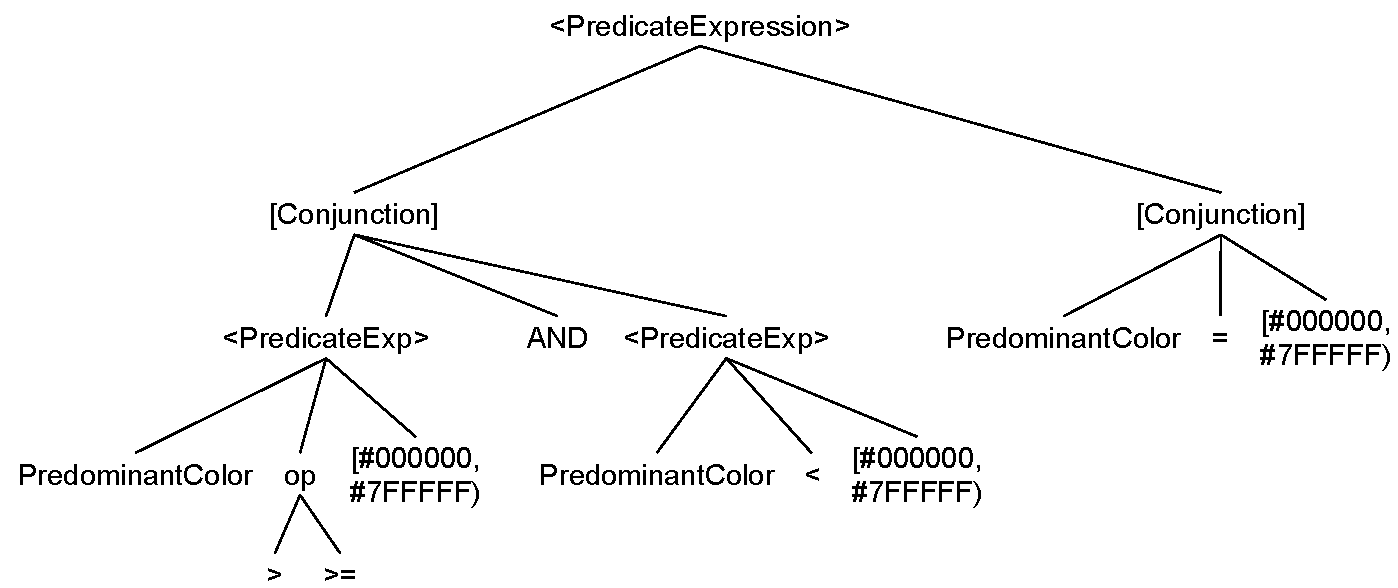
\includegraphics[width=\textwidth]{./figures/case_studies/qpt_index_partitioning_terms_1.pdf}%
}

\subfloat[]{%
  \centering
  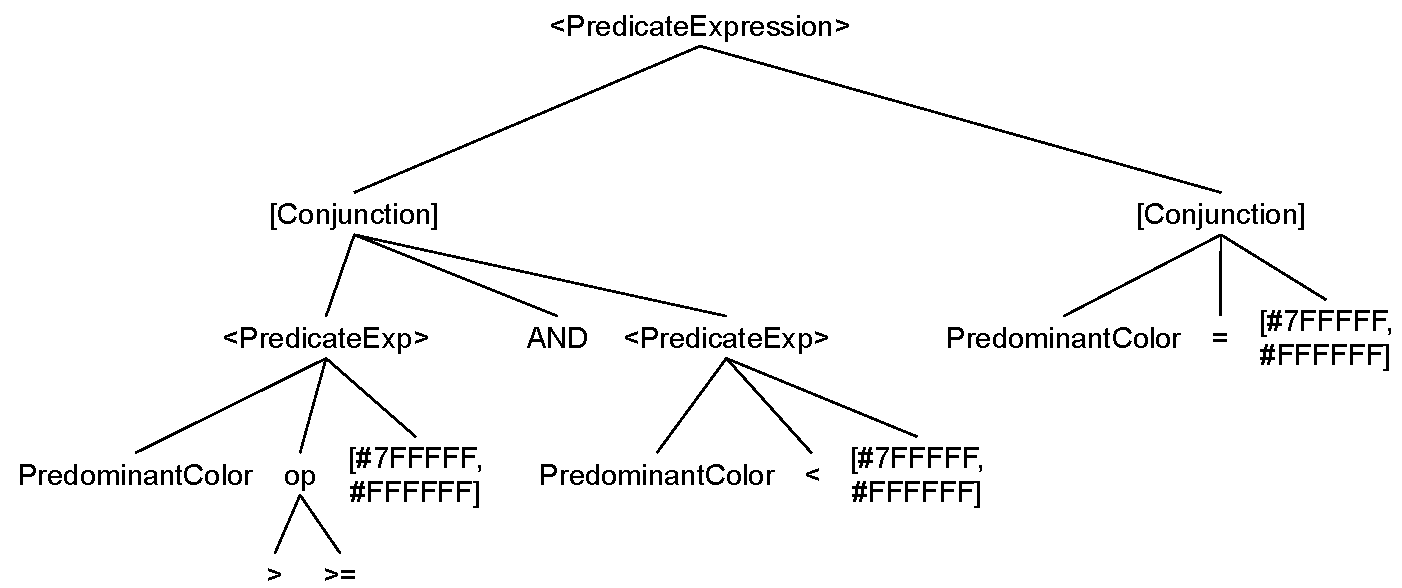
\includegraphics[width=\textwidth]{./figures/case_studies/qpt_index_partitioning_terms_2.pdf}%
}
\caption{The query processing capabilities tree for index partitions $index\_1$ (a) and $index\_2$ (b) of the term-partitioned
index in Figure~\ref{fig:index_partitioned_by_term}}
\label{fig:qpt_index_partitioning_terms}
\end{figure}

\medskip
\noindent
\textbf{Partitioning by term}
Figure~\ref{fig:qpt_index_partitioning_terms} shows the $<predicateExpression>$ subtrees of the QPC tree for $index\_1$ and $index\_2$ in the term-partitioned index QPU
architecture.
The QPC tree of $index\_1$ represents the set of queries in the $[\#000000$, $\#7FFFFF$) interval,
while the QPC tree of $index\_2$ represents the interval $[\#7FFFFF$, $\#FFFFFF$].

Given the query \\
{\obeylines\obeyspaces
Q = SELECT primaryKey, predominantColor
    FROM photoAlbum
    WHERE predominantColor $\geq$ $\#21B1FF$ AND predominantColor $<$ $\#ff7b75$
    INTERVAL FROM LATEST
} ~\\
the intersection between the parse tree of $Q$ the QPC tree of $index_1$ results to the query \\
{\obeylines\obeyspaces
Q1 = SELECT primaryKey, predominantColor
    FROM photoAlbum
    WHERE predominantColor $\geq$ $\#21B1FF$ AND predominantColor $<$ $\#7FFFFF$
    INTERVAL FROM LATEST
} ~\\
and the intersection between the parse tree of $Q$ the QPC tree of $index_2$ results to the query \\
{\obeylines\obeyspaces
Q2 = SELECT primaryKey, predominantColor
    FROM photoAlbum
    WHERE predominantColor $\geq$ $\#800000$ AND predominantColor $<$ $\#ff7b75$
    INTERVAL FROM LATEST
} ~\\
The partition sends a query request for Q1 to $index_1$ and Q2 to $index_2$.
It merges the returned streams and emits the merged stream as its output stream.

In summary, in the term-partitioned index QPU architecture,
for a given query, the partition manager generates and sends downstream queries to index partitions according their corresponding
value intervals, using the QPC tree mechanism.

\medskip
\noindent

Using ... \todo{basically say that the value here is to support select the partitioning scheme during index creation}

It is important to note that DynamoDB \cite{dynamodb:secondaryindexes} and Apache Phoenix \cite{phoenix:secondaryidnexing}
support index partitioning schemes.
However, we believe that the proposed framework provides a more structured approach to the design of query processing system.

Furthermore, the proposed approach is more flexible, as it enables
\todo{add hybrid}



% \section{Materialized views at the edge}
\section{Flexible Materialize view something something}

In this case study, we examine an existing application that requires the use of pre-computed state,
and study how this application can benefit by using QPU-based architecture as a backend.

Lobsters \cite{lobste:rs} is a news aggregator web application.
In Lobsters user post and comment on links (\textit{stories} in the Lobsters terminology).
Moreover, users vote on stories and comments, and votes are used to rank stories.

The Lobsters application is read-heavy.
Traffic data for the production deployment of Lobster, provided by Lobsters' administrators \cite{lobste:stats} 88\% to 97\%
of the users' interactions with the application are operations tha perform reads to the application's backend.
These include viewing specific stories (55\%) and viewing the frontpage (30\%).

In applications such as Lobsters in which read performance is important, application developers often implement mechanisms to optimize it.
Lobsters, in addition to storing individual votes in a votes table, also stores per-story vote counts and story rankings as in separate table columns. \cite{lobsters:schema}
Pre-computing and storing vote count and story rankings avoids the need re-compute them on every page load.
However, the application needs to explicitly update the pre-computed values every time a vote is casted.

Another approach that read-heavy applications employ is to use an in-memory key-value store, such Redis, memcached \cite{nishtala:memcachefacebook}
as a cache to speed up common-case queries.
Using the cache reduces load the database as queries can be served from the cache when the underlying records are unchanged.
The downside is that the application code must explicitly invalidate and replace cache entries as database records change.
This requires complex application-side logic, and is error-prone.

\bigskip
\noindent
In this case study, we focus on a subset of Lobster's functionality that can de modeled as follows:

\begin{lstlisting}[
          language=SQL,
          showspaces=false,
          basicstyle=\ttfamily,
          commentstyle=\color{gray},
          rulecolor=\color{black},
          stringstyle=\color{mymauve},
          frame=L,
          xleftmargin=\parindent
        ]
TABLE users (id int, username text)
TABLE stories (id int, author_id int, title text, url text);
TABLE votes (user_id int, story_id int, vote int);
\end{lstlisting}

\noindent
We demonstrate a QPU architecture that expresses a materialized view which pre-computed the $vote\_count$ for each story
The goal of this view is to facilitate the query that the application executes for loading a requested story:

\begin{lstlisting}[
          language=SQL,
          showspaces=false,
          basicstyle=\ttfamily,
          commentstyle=\color{gray},
          rulecolor=\color{black},
          stringstyle=\color{mymauve},
          frame=L,
          xleftmargin=\parindent,
          commentstyle = \color{gray}
        ]
SELECT id, author_id, title, url, vote_count
FROM stories
JOIN (
  SELECT story_id, SUM(vote) as vote_count
  FROM votes
  GROUP BY story_id
) view
ON stories.id = view.story_id
/* ? is a parameter */
WHERE stories.id = ?
\end{lstlisting}

\begin{figure}[t]
  \centering
    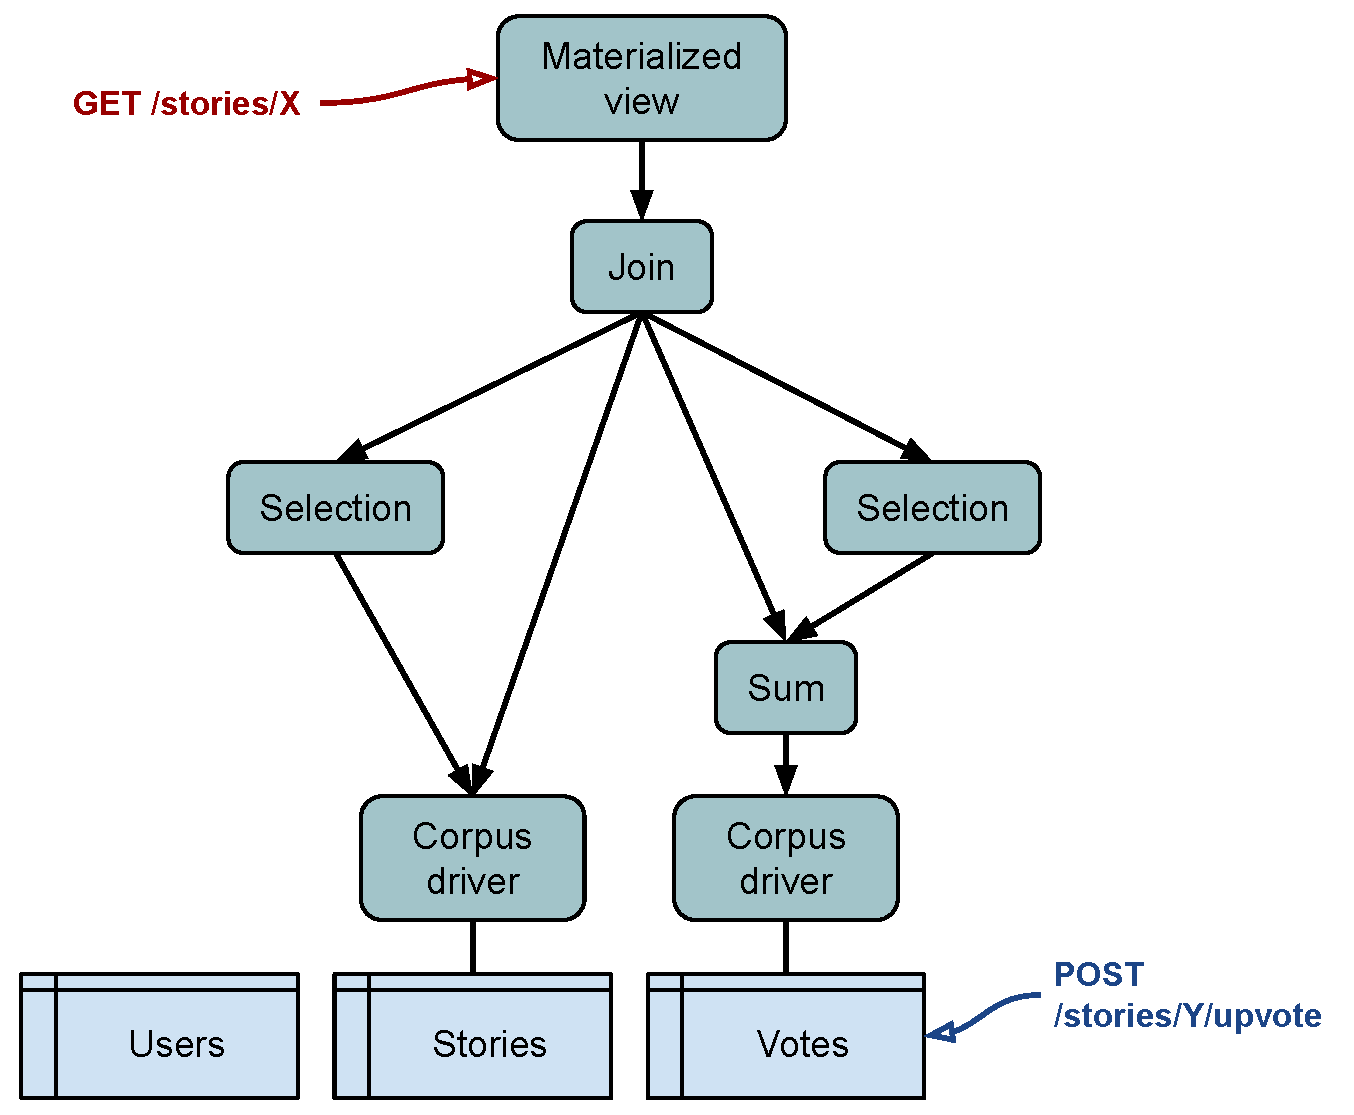
\includegraphics[scale=0.5]{./figures/case_studies/lobsters_architecture_basic.pdf}
  \caption{Lobsters\_architecture\_basic.}
  \label{fig:lobsters_architecture_basic}
\end{figure}

Figure~\ref{fig:lobsters_architecture_basic} shows the QPU architecture that provides this functionality.
We use a \textbf{Sum} QPU for calculating the $vote\_count$ for each story.
It's query processing interface domain consists of a single query:

\begin{lstlisting}[
          language=SQL,
          showspaces=false,
          basicstyle=\ttfamily,
          commentstyle=\color{gray},
          rulecolor=\color{black},
          stringstyle=\color{mymauve},
          frame=L,
          xleftmargin=\parindent
        ]
SELECT story_id, SUM(vote)
FROM stories votes
SNAPSHOT LATEST
INTERVAL FROM LATEST
\end{lstlisting}

Given this query, the Sum QPU's query processing function sends a downstream query to the votes $corpus\_driver$
in order to receive the most recent snapshot of the votes table
and subscribe to subsequent writes to the table.
It receives an input stream consisting of each record in the votes table snapshot,
and incrementally calculates the sum of the $vote$ attribute ($vote\_count$) for each distinct $story\_id$.
It stores $(story\_id$, $vote\_count)$ tuples at its state.
When it completes processing the snapshot, the Sum QPU emits all $(story\_id$, $vote\_count)$ tuples at its response stream.
At the same time, the Sum QPU also receives an input record for each insert to the votes table.
Any update record received while still processing the snapshot, is treaded as a snapshot record;\
It updates corresponding $vote\_count$ but does not result to an output record.
For Each update received after the votes table snapshot has been processed, the Sum QPU updates the $vote\_count$ for the
corresponding $story\_id$,
and emits the updated $vote\_count$ at the output stream.

\begin{figure}[t]
  \centering
    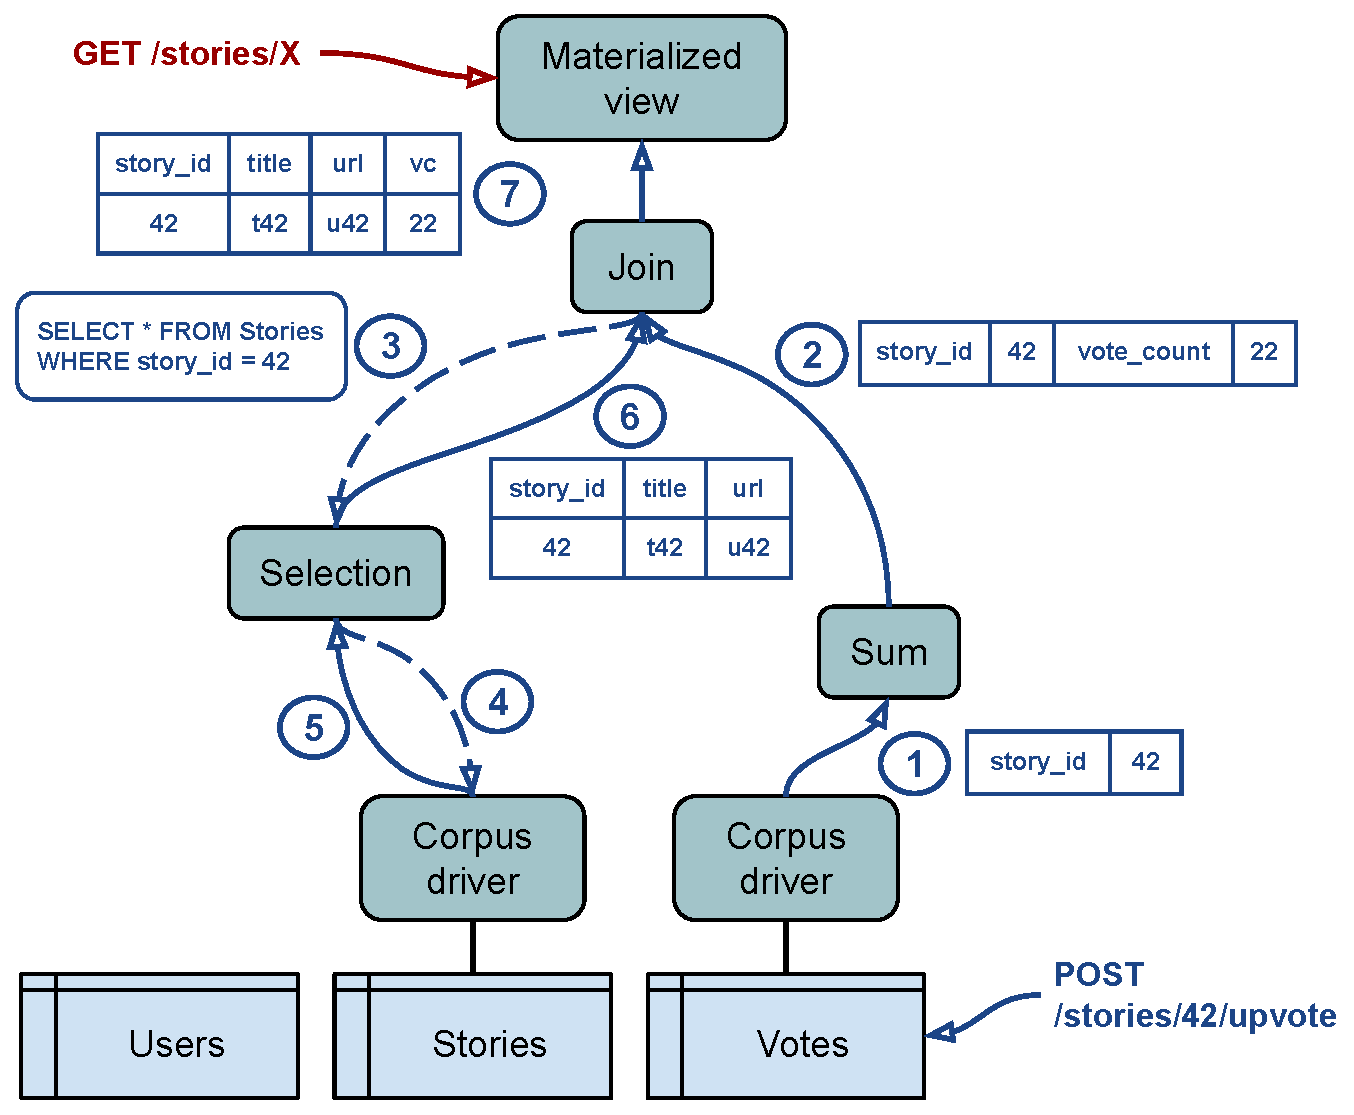
\includegraphics[scale=0.5]{./figures/case_studies/lobsters_architecture_basic_vote.pdf}
  \caption{Lobsters\_architecture\_basic\_vote}
  \label{fig:lobsters_architecture_basic_vote}
\end{figure}

\medskip
\noindent
Moreover, we use a Join QPU in order to join $vote\_count$ with the rest of the attributes of each story.
In the case study, we use a \textit{stateless} Join QPU.
This Join QPU does not store intermediate state of its inputs.
When it receives a query,
its query processing function sends a persistent query to each $corpus\_driver$ QPUs in order to establish input streams
for receiving notifications for updates to the corresponding tables.
As shown in Figure~\ref{fig:lobsters_architecture_basic_vote},
for $(story\_id$, $vote\_count)$ tuple that the Join QPU receives from the votes $corpus\_driver$,
it performs a query to the $Selection$ QPU connected to the stories table, requesting the record with the corresponding $story\_id$.
It then joins the received record with the $vote\_count$, and emits the join result at the output stream.

Similarly, for each $(story\_id$, $author\_id$, $title$, $url)$ tuple received from the stories table,
the Join QPU sends a downstream query to $Selection$ QPU it is connected to in order to retrieve the corresponding $vote\_count$.

\medskip
\noindent
Finally, a Materialized View QPU is connected to the Join QPU.
It is responsible for storing the result of the join operation, and serving queries of the form

\begin{lstlisting}[
          language=SQL,
          showspaces=false,
          basicstyle=\ttfamily,
          commentstyle=\color{gray},
          rulecolor=\color{black},
          stringstyle=\color{mymauve},
          frame=L,
          xleftmargin=\parindent
        ]
SELECT id, author_id, title, url, vote_count
FROM stories_with_voteCount
/* ? is a parameter */
WHERE id = ?
\end{lstlisting}


\medskip
\noindent
In summary,
this QPU architecture provides the functionality of pre-computing story votes counts in order to avoid re-computation
when serving user read requests.
This is equivalent to the functionality already implemented in the Lobsters application.
However, using shifts the responsibility of updating the vote counts from the application logic,
to the query processing architecture, thus simplifying the application code.


\subsection{Partial materialization}

Next, we expand the Lobsters case study be examining the operation of loading the application's frontpage.
The frontpage consists of the $K$ stories with the highest vote count ($K$ being a parameter).

The Lobsters implementation uses the following query to retrieve the information required for loading the frontpage:

\begin{lstlisting}[
          language=SQL,
          showspaces=false,
          basicstyle=\ttfamily,
          commentstyle=\color{gray},
          rulecolor=\color{black},
          stringstyle=\color{mymauve},
          frame=L,
          xleftmargin=\parindent
        ]
SELECT id, author, title, url, vote_count
FROM stories
JOIN (
  SELECT story_id, SUM(v.vote) as vote_count
	FROM votes
	GROUP BY story_id
) view
ON stories.id = view.story_id
ORDER BY vote_count DESC
LIMIT K
\end{lstlisting}

\begin{figure}[t]
  \centering
    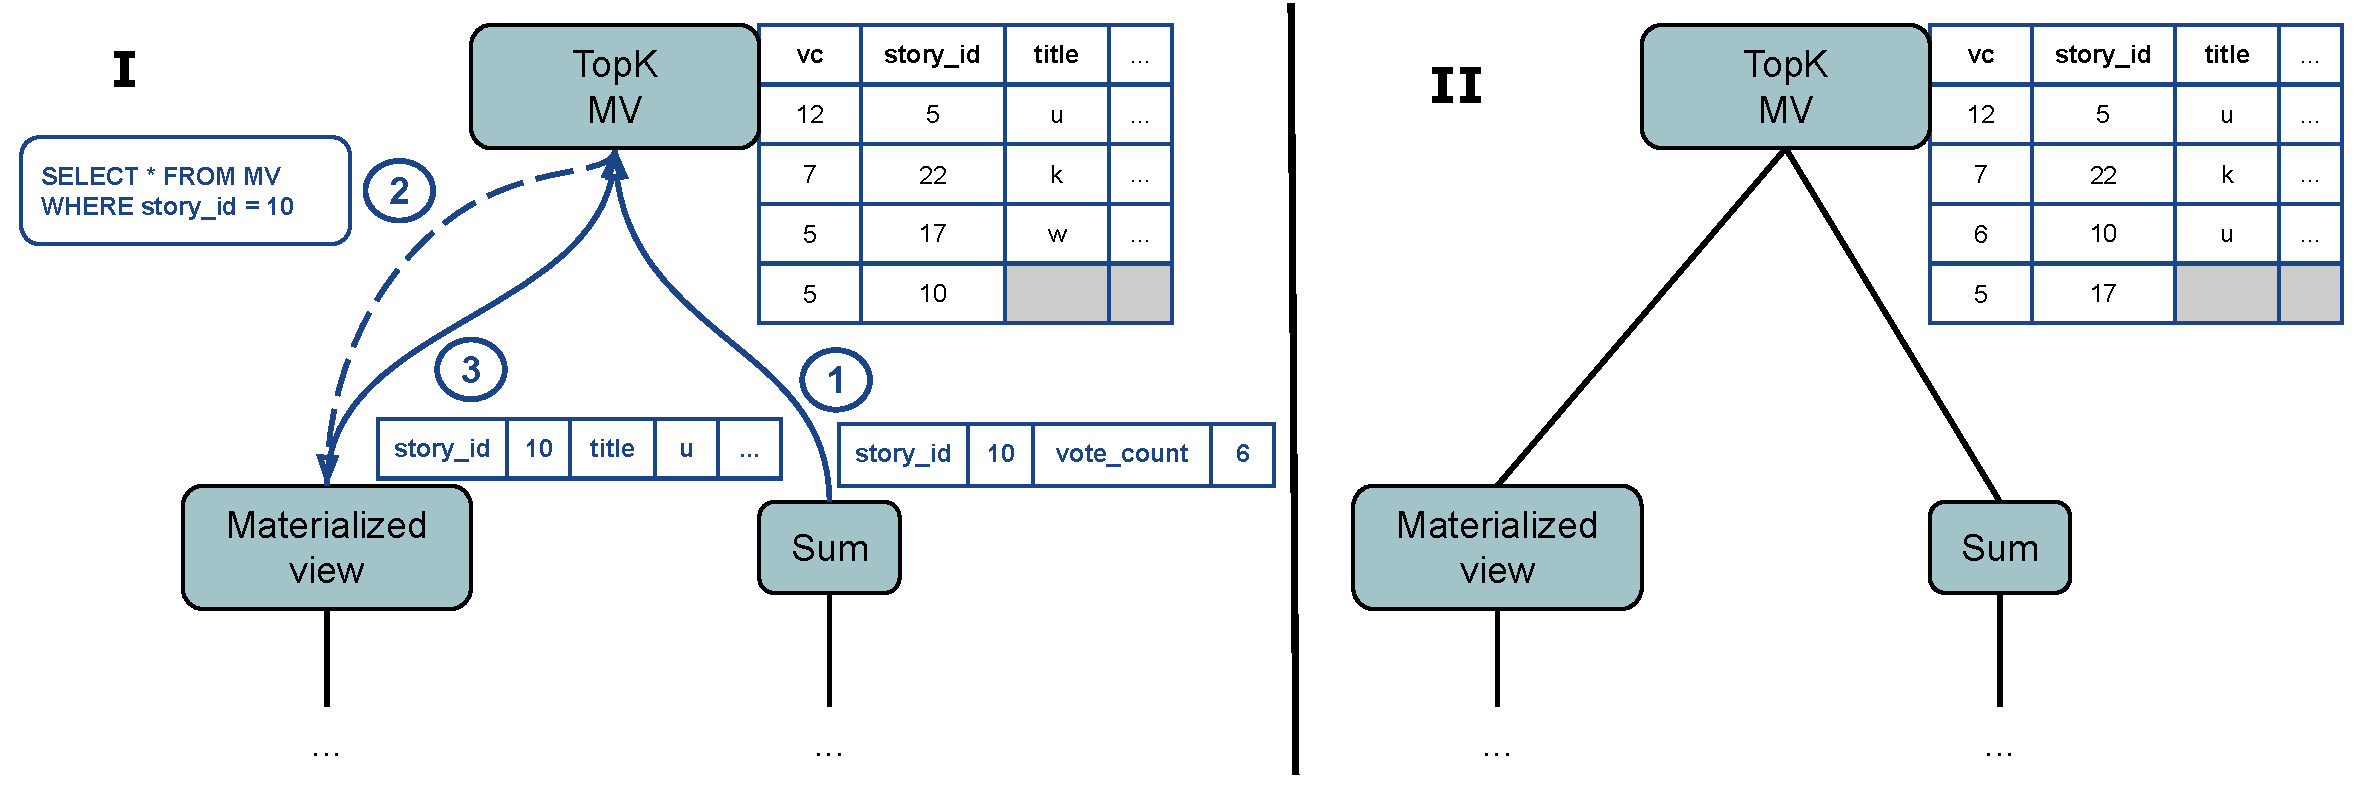
\includegraphics[scale=0.4]{./figures/case_studies/lobsters_architecture_materialization.pdf}
  \caption{Lobsters\_architecture\_materialization}
  \label{fig:lobsters_architecture_materialization}
\end{figure}

In this section, we show how the QPU architecture defined in the previous section can be extended to provide this
functionality.

To achieve that, we introduce an additional query processing unit class: the TopK Materialized View (TopK-MV) QPU.
The TopK-MV is represents a materialized view which orders its entries based on a specified attribute,
and only materializes the entries with the $K$ highest (or lowest, based on the configuration) values for that attribute.

We deploy a TopK-MV QPU in the Lobster application QPU architecture (Figure~\ref{fig:lobsters_architecture_materialization}),
and configure it as a materialized view with the same definition as the existing materialized view,
storying entries of the form $(story\_id$, $author\_id$, $title$, $url$, $vote\_count)$.
In addition, we configure TopK-MV QPU to order entries by $vote\_count$, and materialize the $K$ entries with the highest $vote\_count$.

The TopK-MV is connected to the materialized view and the Sum QPU.
Its initialization function sends a persistent query to the Sum QPU.
As a result, it first receives a snapshot containing the $vote\_count$ of every existing story,
and then continues receiving an update for each change to the $vote\_count$ of a story.
It stores the received snapshot as a list of $(vote\_count$, $story\_id)$ entries, ordered by $vote\_count$.
Then for each of the $K$ entries with the highest $vote\_count$,
it queries the materialized view in order to retrieve the remaining attributes of the corresponding story.
Therefore, the TopK-MV \textit{materializes} only a specified number of entries,
based on a certain criterion.

Furthermore, the TopK-MV QPU continues receiving updates from the Sum QPU, and updating its
ordered list of $(vote\_count$, $story\_id)$ entries.
When the $vote\_count$ of a non-materialized entry becomes one of the top-K,
the unit's callback function discards the materialized entry with the lowest $vote\_count$,
and triggers the materialization of that entry.

The Top-K QPU uses the technique of \textit{partial-materialization} in order to bound the size of pre-computed state.
This is a well known concept for materialized views in database systems \cite{zhou:partiallymaterialized, zhou:dynamicmaterialized},
and has been used by Noria \cite{gjengset:noria} in the context of data-flow systems.

\subsection{Edge something something}

% The ad-serving application's users are distributed worldwide, and therefore, the communication latency between user devices and the data center may be significant.
% Placing data geographically closer to end users is a common technique for reducing the large access latencies resulting from geo-distribution 

Query response time is crucial for in user-facing read-heavy application, such as Lobsters.
As discussed in chapter~\ref{ch:background}, even small increases in user-perceived latency can result in significant drops in both web traffic and sales.
So far in this case study, we have examined how query processing latency can be decreased using pre-computed query results.
Another factor contributing to large query processing latencies is the communication latency between the application and the clients.
A client located in a different geographic region than the Lobsters application deployment might experience communication
latency with the application backend in the order of hundreds of milliseconds.

A common solution to this latency problem is to place on servers geographically closer to clients using caches,
in order to avoid costly remote round-trips to data centers.
These servers, called edge nodes, are a crucial component in industry architectures.
For example, Google operates comparatively few data centers relative to edge nodes \cite{google:infra}.
In existing applications,
edge nodes are largely used for caching static data, such as images and video content, for example in content delivery network architectures.

\begin{figure}[t]
  \centering
    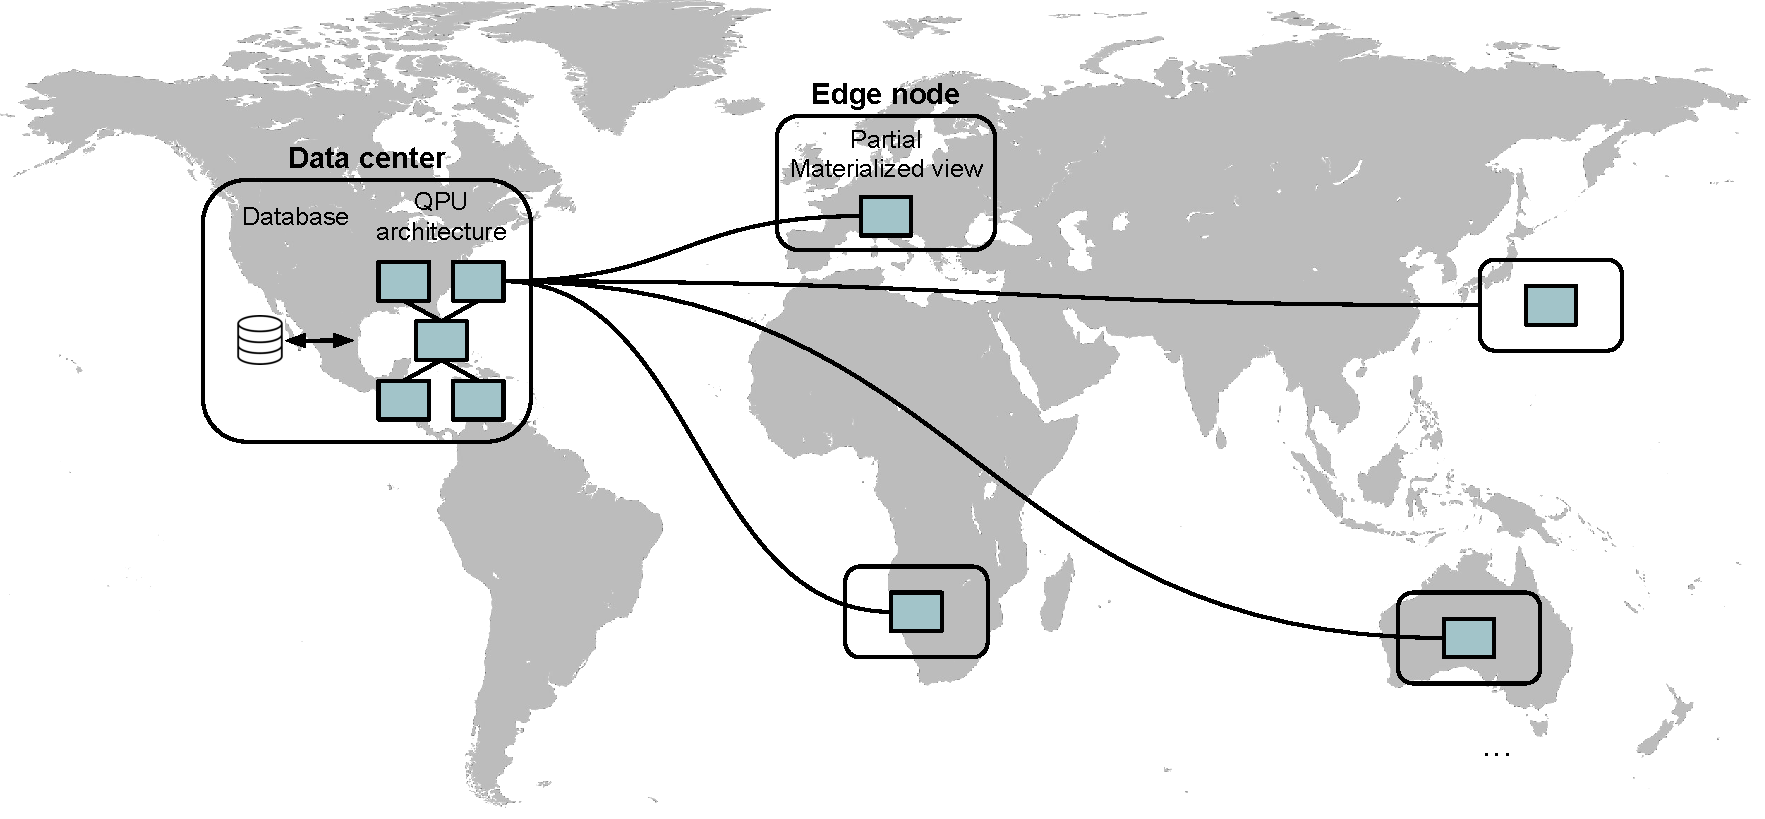
\includegraphics[scale=0.4]{./figures/case_studies/lobsters_architecture_edge.pdf}
  \caption{Lobsters\_architecture\_edge}
  \label{fig:lobsters_architecture_edge}
\end{figure}

\medskip
\noindent
Because of its modularity, the proposed query processing architecture can be used to place derived state, such as materialized views,
closer to client.
More specifically,
the query architecture designed for the Lobsters application (Figure~\ref{fig:lobsters_architecture_materialization}) can be
distributed among the data centers and edge nodes.
Considering a system architecture composed of a data center and multiple edge nodes,
we can place a TopK Materialized View QPU on each edge node, as shown in Figure~\ref{fig:lobsters_architecture_edge}.
Each TopK-MV QPU stored pre-computed state for the $K$ stories with the most votes.
It thus provides low latency access to the data required for loading the application's frontpage,
while maintaining a bounded memory footprint.
We connect each TopK-MV QPU to the complete Materialized View QPU and the SUM QPU placed in the data center,
In that way, TopK-MV QPUs can receive updates for updated vote counts,
and also request the materialize new stories as the reach the application frontpage.

We configure the connections between each TopK-MV QPU and the QPU architecture placed on the data center to be asynchronous,
as propagating each vote to the edge nodes synchronously adds a significant overhead to vote operations.
This choice makes a trade-off between write latency and the freshness of materialized views.
Propagating updates to materialized views asynchronously means that views are eventually consistent,
and might therefore return stale results.

In chapter~\ref{ch:evaluation}, we evaluate the effect of placing materialized view closer to clients on query response time and
and query result freshness.

\section{Federated secondary attribute search for multi-cloud object storage}

\begin{figure}[t]
  \centering
    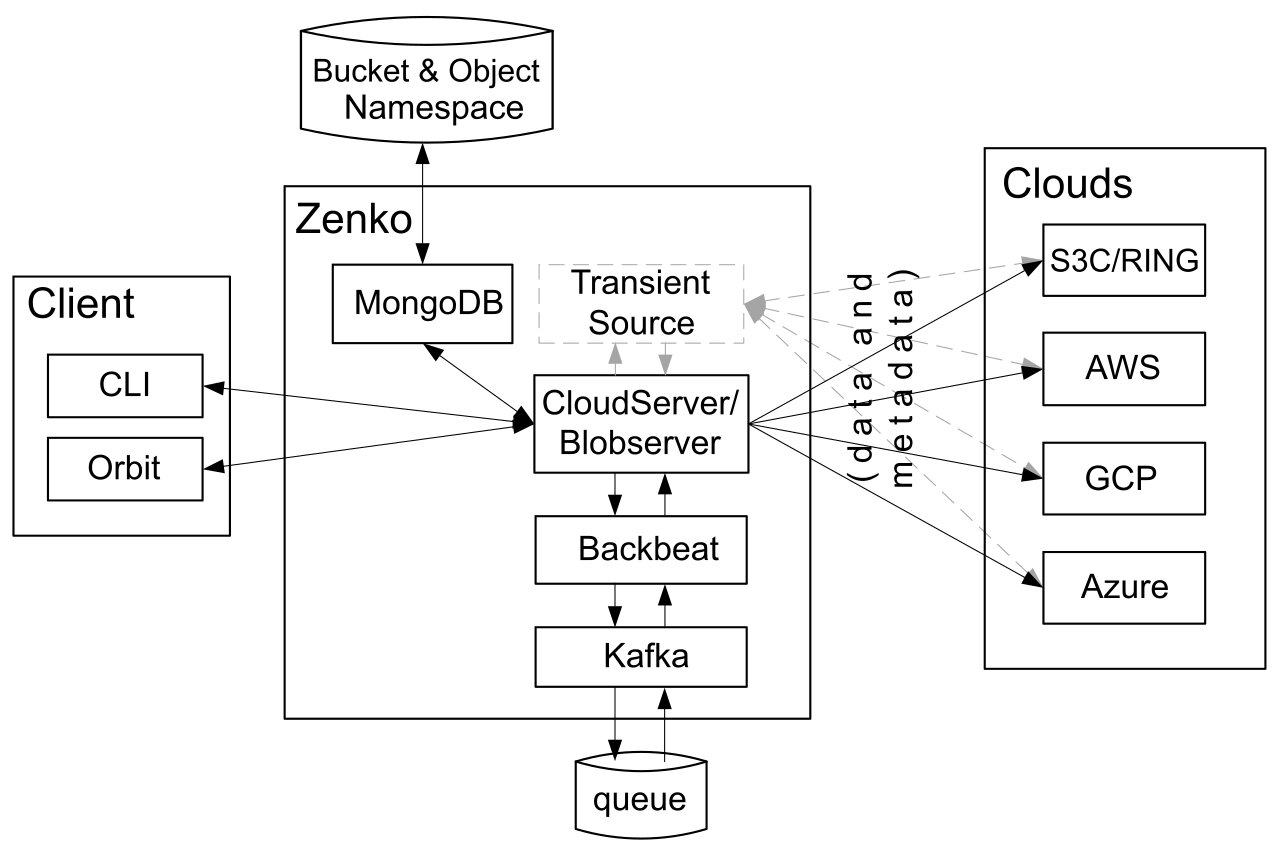
\includegraphics[scale=0.3]{./figures/case_studies/zenko_arch.jpg}
  \caption{zenko\_arch}
  \label{fig:zenko_architecture}
\end{figure}

While most enterprise data today originate from and is stored on-premises storage systems,
use cases for hybrid and multi-cloud storage are emerging in many industries.
For example, in the media industry, while the creation of content in on-premises private clouds is prevalent,
the use of public cloud services for content distribution and transcoding \cite{scality:bloomberg} is growing.
Moreover, organization increasingly choose to spread their data across multiple cloud providers in order to avoid
dependence on a single provider, and improve their resilience against failures.

The advent of data distributed across multiple independent storage platforms has created the need for unified access to data across platforms.
In this section, we examine a Zenko \cite{zenko:docs}, a multi-cloud data controller that aims to address this need.
Zenko provides a unified namespace, API, and search capabilities for data stored locally,
or in public cloud storage services, including Amazon S3, Microsoft Azure Blob storage, and Google Cloud Storage.
We focus on Zenko's search capabilities.

Zenko provides a common namespace over a set of distinct storage platforms, and supports an object storage API \cite{aws:s3}.
It is common for application to mark objects with metadata tags.
Zenko provides federated metadata search:
applications can retrieve objects through searches on their metadata tags, independent from their storage location.

Figure\ref{fig:zenko_architecture} show Zenko's architecture.

% application can search objects based thier 
% There exists thus a need for a centralized abstraction of multiple storage services, either on-premise or 3rd party objects torage infrastructure platforms

% More recently, the concept of multi-cloud data storage has emerged.
% Organizations spread their data across private data centers and public cloud services in order to reduce costs and
% ensure fault-tolerance.
% Moreover, they distribute data across multiple cloud providers in order to avoid dependence on a single
% cloud provider, take advantage of diverse storage and computing services, and improve reliability.



% Scality’s open source multi-cloud framework, Zenko 1, enables applications to transparently store and access data on multiple public and private cloud storage systems using a single storage interface. Applications can use Zenko to access multiple cloud storage systems, including cloud services such as Microsoft Azure Blob Storage, Amazon S3 and Google Cloud, as well as private on-premise storage systems, using an Amazon S3 compatible API.
% The focus of this use case is Zenko’s capability to support federated metadata search across multiple cloud namespaces. This enables applications to retrieve data by perform- ing queries on metadata attributes, independent of the data location.

%%
In this case study, examines one of Scality's technologies and proposes alternative approaches.
%%

\bibliographystyle{plainnat}
\bibliography{refs}